\documentclass[12pt]{report}

\usepackage[left=1in, right=1in, top=1in, bottom=1in]{geometry}

\usepackage{xcolor}
\usepackage{graphicx}
\usepackage{multicol}
\setlength\parindent{0pt}

\usepackage{graphicx, amsmath,anonchap,tabularx, multicol,verbatim}

\usepackage{enumitem,mdwlist}
\setlist{noitemsep}
\setlist{nolistsep}

\newenvironment{boxe}
    {\begin{center}
    \begin{tabular}{|p{0.9\textwidth}|}
    \hline\\
    }
    { 
    \\\\\hline
    \end{tabular} 
    \end{center}
    }

\begin{document}
\begin{tabular*}{\textwidth}{@{\extracolsep{\fill}}ll}
\textbf{Math 160} The limit definition of a derivative & \;\;Name: \hrulefill \\
 Hughes-Hallet Chapter 2& Derivatives and derivative rules\hspace{1in}  \\
\hline\hline
\end{tabular*} \\

\pagenumbering{gobble}


\begin{boxe}  \textbf{The Definition of a Derivative:} The derivative of $f(x)$ at $x=a$, is defined as 
$$f'(a)=\lim_{h\to 0}\frac{f(a+h)-f(a)}{h}$$
The derivative function of $f(x)$ is defined as
$$f'(x)=\lim_{h\to 0}\frac{f(x+h)-f(x)}{h}$$
The derivative function can be written as $f'(x)=\dot{f}(x)=\frac{d}{dx}\left[f(x)\right]=\frac{df}{dx}(x)$ and the derivative at a point can be written as $f'(a)=\frac{d}{dx}\left[f(x)\right]_{x=a}=\frac{df}{dx}\big|_{x=a}$
\end{boxe}

\begin{boxe}
\textbf{Constant Rule:} $\displaystyle{\frac{d}{dx}\left[c\right]=0}$\;\;\;\;\;\;\;\;\;\;\textbf{Power Rule:} $\displaystyle{\frac{d}{dx}\left[x^n\right]=nx^{n-1}}$\\
\textbf{Coefficient Rule:} $\displaystyle{\frac{d}{dx}\left[c\cdot f(x)\right ]}=\displaystyle{c\cdot \frac{d}{dx}\left[f(x)\right]}$\\
\textbf{Addition Rule:} $\displaystyle{\frac{d}{dx}\left[f(x)+g(x)\right]}=\displaystyle{\frac{d}{dx}\left[f(x)\right]+\frac{d}{dx}\left[g(x)\right]}$
\end{boxe}

\begin{enumerate}
\item Using the rules above, show that $\displaystyle{\frac{d}{dx}\left[f(x)-g(x)\right]}=\displaystyle{\frac{d}{dx}\left[f(x)\right]-\frac{d}{dx}\left[g(x)\right]}$\\\\\\\\\\\\

\item Simplify the following functions and find their derivative functions using the rules above

\begin{enumerate}[label=\alph*.]
    \item $\displaystyle{\sqrt[5]{x^{3}}}$\\\\\\
    \item $\displaystyle{\frac{3}{\sqrt[3]{x}}}$\\\\\\\\
    \item $\displaystyle{\frac{1}{2}x^{-\frac{3}{4}}}+x^{99}$
\end{enumerate}
\newpage
\item Draw examples of each of the 4 types of discontinuities. And for each determine (i) the type of discontinuity,  derivative at the point of the discontinuity 
\end{enumerate}
\begin{minipage}{0.48\textwidth}
     \centering
     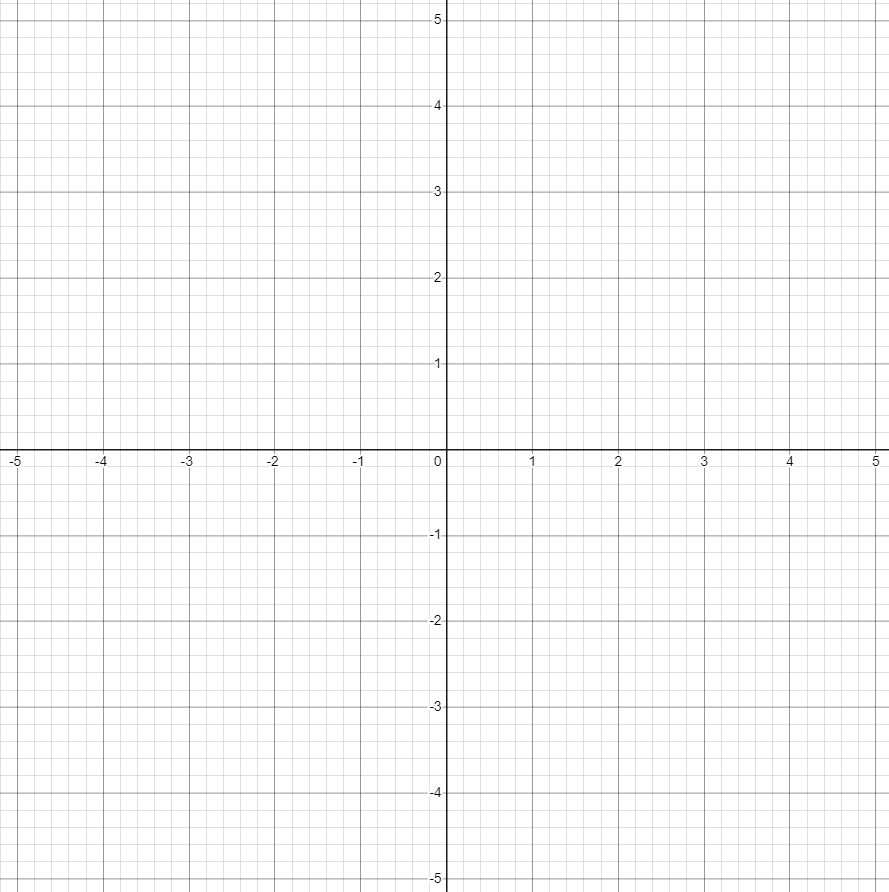
\includegraphics[width=.9\linewidth]{emptyplot.png}
     \begin{enumerate}[label=\alph*.]
         \item Name the Discontinuity
         \item At what $x$-value(s) is your function discontinuous: 
         \item Graphically 
     \end{enumerate}
   \end{minipage}\hfill
   \begin{minipage}{0.48\textwidth}
     \centering
     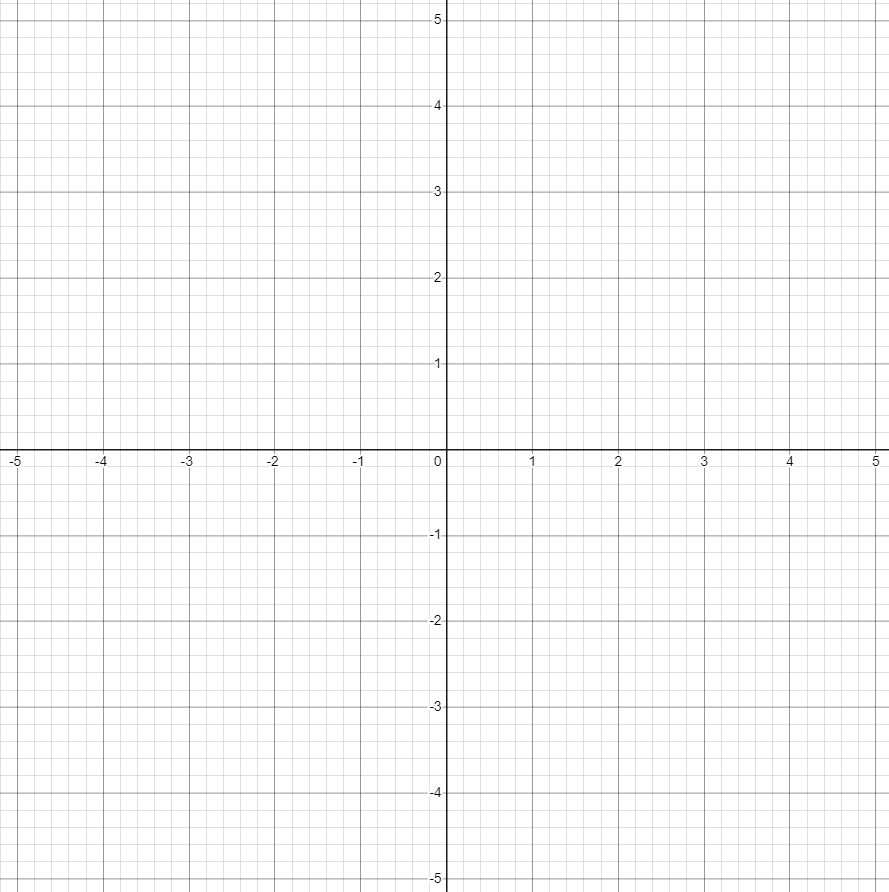
\includegraphics[width=.9\linewidth]{emptyplot.png}
   \end{minipage}

\begin{minipage}{0.48\textwidth}
     \centering
     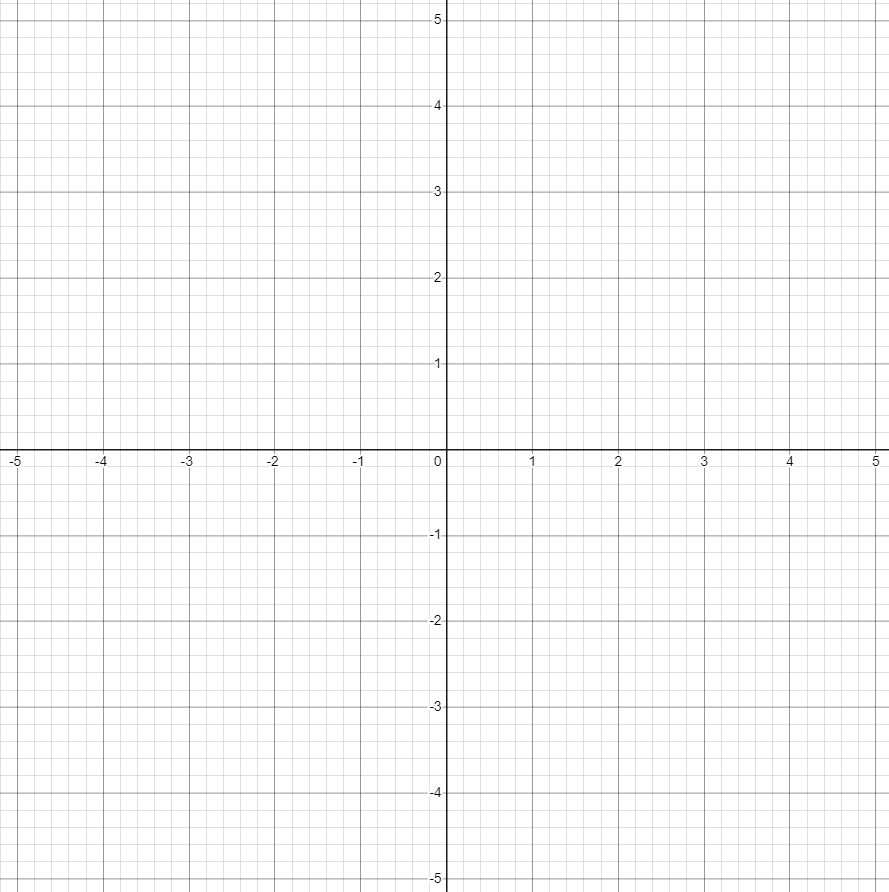
\includegraphics[width=.9\linewidth]{emptyplot.png}
   \end{minipage}\hfill
   \begin{minipage}{0.48\textwidth}
     \centering
     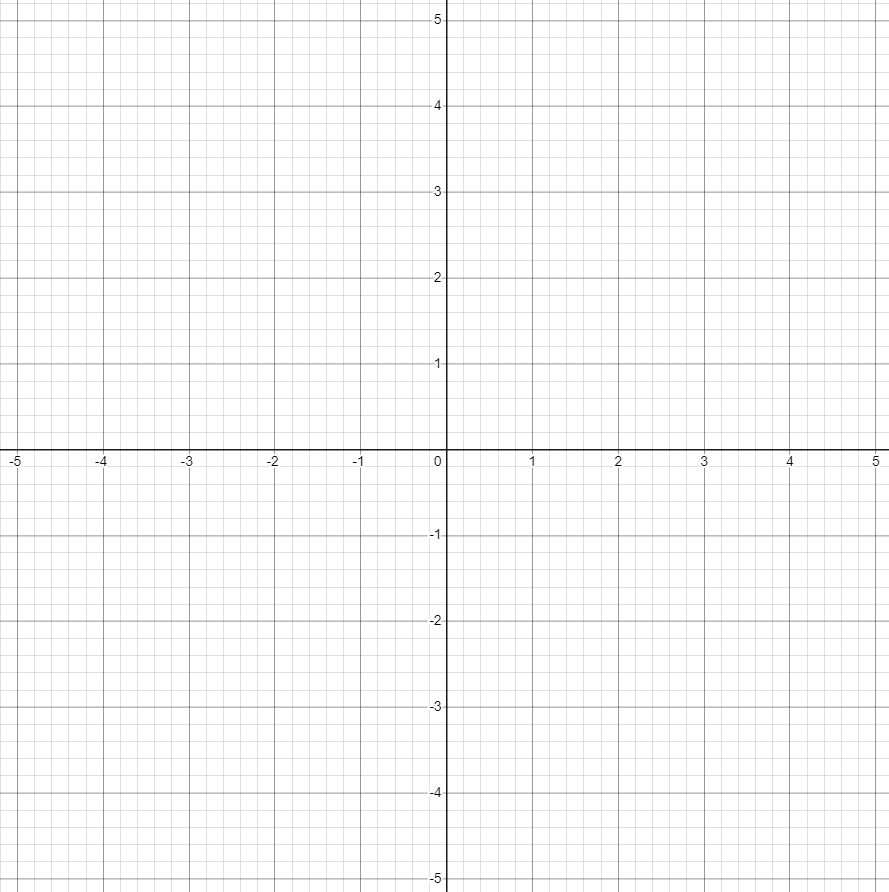
\includegraphics[width=.9\linewidth]{emptyplot.png}
   \end{minipage}








\end{document}
